\section{ART Model}
\label{sec:model}

\begin{figure}[htbp]
	\hspace{0ex}
	\vspace{0ex}
	\centering
	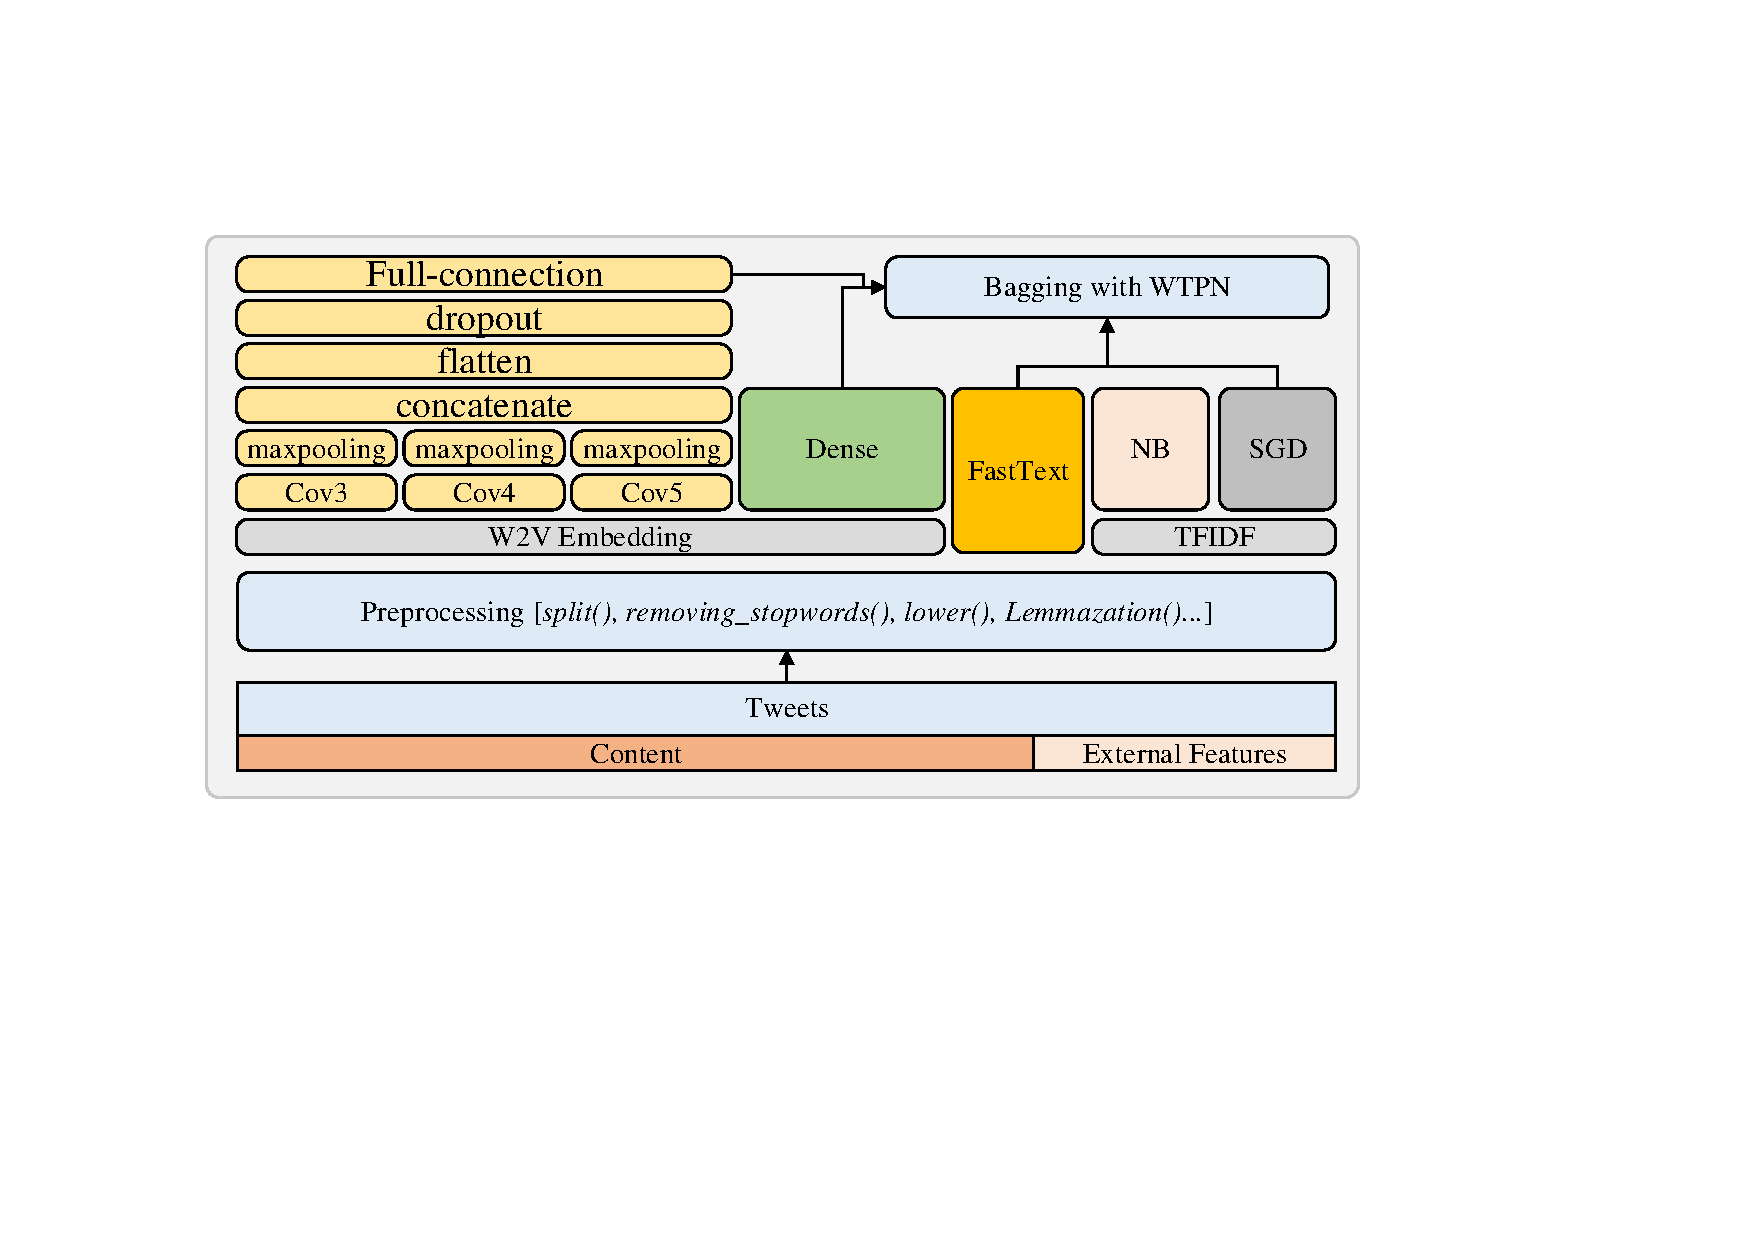
\includegraphics[width = \textwidth]{fig/structure}
	\caption{Architecture of ART}
	\label{fig:architecture}
\end{figure}

\subsection{Aggregated Model}
\label{sec:aggregated_model}
Aggregated model is a mixture model that consists of several different components. For a particular job, several basic models can achieve it. If we combine them, the aggregated performance is usually better than that of a single model. Also, for different types of features, the most suitable classifier is changing. Consequently, using the aggregated model can effectively promote the performance of rumor tracking. 

\subsection{Architecture}
\label{sec:architecture}
The architecture of ART is shown in Fig.\ref{fig:architecture} . As we can see, the input of  ART consists of two types of features, including content features and social features. Then, all features will be embedded and be sent to filters or classifiers.  Some components such as TextCNN or Dense use word-to-vector embeddings and the other components use their embedding methods. Next, each trained component will make its prediction respectively. Finally, we add the predictable results of all components and give the final prediction by a voting aggregated strategy.

\subsection{Preprocessing and Embedding}
\label{sec:process_embedding}
Content is the text of the tweet, which is the most important feature for the rumor tracking task. The text of the tweet is short, which is restricted within 140 words. Usually, the spelling in tweets is causal with symbols mixed in it. Consequently, before input them into the model, we will conduct prepossessing firstly. The prepossessing in NLP is roughly immobilized, we only need to make some minor adjustments. In this work, we adopt splitting on tweets, then removing the punctuation and special characters. Next, we turn all characters into lowercase. Finally, we adopt lemmatization on all words.

High-quality embedding of text is a key factor for NLP tasks. Generally speaking, we have three embedding strategies: pre-trained embedding, trained embedding on the current dataset, and random embedding. Pre-trained embedding is trained on a corpus with very big scales, and some of the famous ones are GloVe \cite{DBLP:conf/emnlp/PenningtonSM14}, Google News embedding\cite{DBLP:journals/corr/abs-1301-3781}. It is common practice to train embedding on the current dataset, and we also do this in PHEME and RumorEval dataset. The last way is using random embedding, which assigns each word with a unique embedding randomly. In this work, we try all three embedding strategies and the detailed performance will be introduced in section \ref{sec:experiment}. By comparing them, we finally choose random embedding as the strategy in ART.

\begin{algorithm}[tbp]
	\caption{Voting based ART}
	\label{algorithm:art}
	\LinesNumbered % show line numbers
	\KwIn{$K_y = \left\{y_F', y_T', y_B', y_N', y_S' \right\}$: outputs of all components;}
	\KwOut{$R$: predictable result of ART;}
	\textbf{Initialize:} Outputs of ART: $y' = [0]*m$, $R = 0$ \;
	
	\For{$y_i'$ in $K_y$}{
		$r = 0$\;
		$r = argmax(y_i')$\;
		$y'[r] ++$;
	}
	
	$R = argmax(y')$
\end{algorithm}

\subsection{Procedure of ART}
After embedding, we send \textbf{content features} to different types of deep learning models. As shown in Fig.~\ref{fig:architecture}, we add TextCNN, SGD, and FastText to dispose of the content feature. These three components are trained respectively until getting convergence. When predicting, each component outputs an m-dimensional vector after the softmax layer. Each dimension suggests the probability that the content belongs to this classification. Despite some content features, the tweets contain plenty of \textbf{social features}. As introduced in section \ref{sec:problem}, we should not get any information about the tweet's branch or threads in advance. Consequently, we omit some features that contain external branch information. Finally, we choose "screen name" and "hashtag" as the social features in ART. 

With all components trained, we aggregate them and give the final prediction on the rumor tracking task. Generally, there are two commonly used aggregation methods: \textbf{joint training} and \textbf{respective training}. Joint training means all models have one shared optimization function, and all parameters are updated together. When predicting, the aggregated model directly outputs the final prediction. Respective training means we train each component respectively. When predicting, each component makes its prediction result. In ART, all results are aggregated by a voting strategy. It means that each component votes to a category and the category with the most votes is the final prediction result. The aggregation details of ART is shown in Algorithm.~\ref{algorithm:art}.
